% The edge selection machine of a color combination (Figure 1 of the paper).
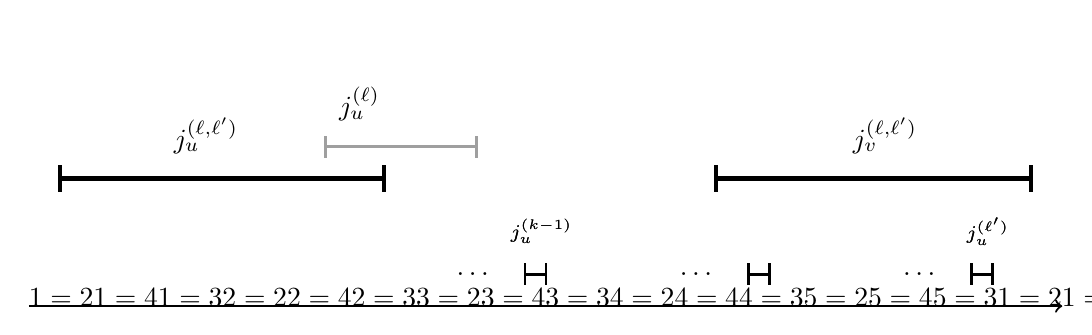
\begin{tikzpicture}[scale=0.75,yscale=1.8]
\def\eps{0.1}
\def\shiftx{5}
\colorlet{grayed}{gray!75}

    \draw[thick,->] (0,0) -- (17.5,0);

    \draw[line width=1.5, |-|] ({0.5}, 1.2) -- (6.05, 1.2);
    \node at (3, 1.6) {$j_u^{(\ell,\ell')}$};

    \draw[line width=1.5, |-|] ({\shiftx+6.6}, 1.2) -- (7+\shiftx+5, 1.2);
    \node at (\shiftx+7+2.5, 1.6) {$j_v^{(\ell,\ell')}$};

    % the vertex jobs of u
    \draw[line width=1,grayed, |-|] (5, 1.5) -- (7.6, 1.5);
    \node at (5.6, 1.9) {$j_u^{(\ell)}$};
    \foreach \x\i\label in {0/1/$j_u^{(k-1)}$, 1/2/$ $, 2/3/$j_u^{(\ell')}$, 3/4/$ $, 4/5/$j_u^{(0)}$}
    {
        \ifthenelse{\(\i=2 \OR \i=4\)}
        {
            \node at (\eps+5+2*\x/5+\eps*\x+0.23, 0.3) {$\dots$};
        }
        {
            \ifthenelse{\(\NOT \i=3\)}
            {
            \draw[line width=1, grayed, |-|]
            (\eps+5+2*\x/5+\eps*\x, 0.3) -- (\eps+5+2*\x/5+0.4+\eps*\x, 0.3);
            \node at (\eps+5+2*\x/5+\eps*\x+0.3, 0.7) {\scriptsize\label};
            }
            {
            \draw[line width=1, |-|]
            (\eps+5+2*\x/5+\eps*\x, 0.3) -- (\eps+5+2*\x/5+0.4+\eps*\x, 0.3);
            \node at (\eps+5+2*\x/5+\eps*\x+0.3, 0.7) {\scriptsize\label};
            }
        }
    }

    % the vertex jobs of v
    \draw[line width=1,grayed, |-|] (5+\shiftx, 1.5) -- (7.5+\shiftx, 1.5);
    \node at (7.0+\shiftx, 1.9) {$j_v^{(\ell')}$};
    \foreach \x\i\label in {0/1/$j_v^{(k-1)}$, 1/2/$ $, 2/3/$j_v^{(\ell)}$, 3/4/$ $, 4/5/$j_v^{(0)}$}
    {
        \ifthenelse{\(\i=2 \OR \i=4\)}
        {
            \node at (\shiftx+\eps+5+2*\x/5+\eps*\x+0.23, 0.3) {$\dots$};
        }
        {
            \ifthenelse{\(\NOT \i=3\)}
            {
            \draw[line width=1, grayed, |-|]
            (\shiftx+\eps+5+2*\x/5+\eps*\x, 0.3) -- (\shiftx+\eps+5+2*\x/5+0.4+\eps*\x, 0.3);
            \node at (\shiftx+\eps+5+2*\x/5+\eps*\x+0.3, 0.7) {\scriptsize\label};
            }
            {
            \draw[line width=1, |-|]
            (\shiftx+\eps+5+2*\x/5+\eps*\x, 0.3) -- (\shiftx+\eps+5+2*\x/5+0.4+\eps*\x, 0.3);
            \node at (\shiftx+\eps+5+2*\x/5+\eps*\x+0.3, 0.7) {\scriptsize\label};
            }
        }
    }

    % the edge job
    \draw[line width=1, |-|] (6.5, 2) -- (11., 2);
    \node at (8.5, 2.4) {$j_{\{u,v\}}$};
\end{tikzpicture}
